\begin{figure}[H]
\begin{center}
	
	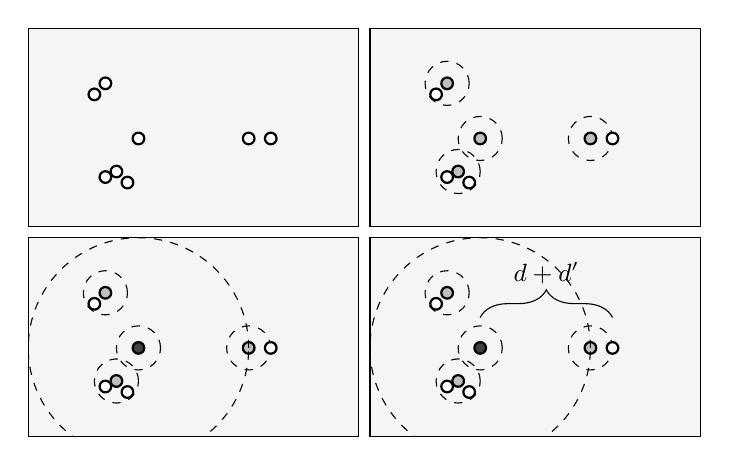
\begin{tikzpicture}[scale=1.4]
	\begin{scope}[]
	\fill[lightgray!15,draw=black] (-1,-0.8) rectangle (2,1);
	\fill[white,draw=black,thick] (0,0) circle (1.5pt);
	\fill[white,draw=black,thick] (1,0) circle (1.5pt);
	\fill[white,draw=black,thick] (1.2,0) circle (1.5pt);
	
	\fill[white,draw=black,thick] (-0.3,0.5) circle (1.5pt);
	\fill[white,draw=black,thick] (-0.4,0.4) circle (1.5pt);
	\fill[white,draw=black,thick] (-0.2,-0.3) circle (1.5pt);
	\fill[white,draw=black,thick] (-0.1,-0.4) circle (1.5pt);
	\fill[white,draw=black,thick] (-0.3,-0.35) circle (1.5pt);
	\end{scope}
	\begin{scope}[shift={(3.1,0)}]
	\fill[lightgray!15,draw=black] (-1,-0.8) rectangle (2,1);
	\fill[lightgray,draw=black,thick] (0,0) circle (1.5pt);
	\fill[lightgray,draw=black,thick] (1,0) circle (1.5pt);
	\fill[lightgray,draw=black,thick] (-0.2,-0.3) circle (1.5pt);
	\fill[lightgray,draw=black,thick] (-0.3,0.5) circle (1.5pt);
	
	\draw[dashed] (0,0) circle (0.2);
	\draw[dashed] (1,0) circle (0.2);
	\draw[dashed] (-0.2,-0.3) circle (0.2);
	\draw[dashed] (-0.3,0.5) circle (0.2);
	
	\fill[white,draw=black,thick] (1.2,0) circle (1.5pt);
	\fill[white,draw=black,thick] (-0.4,0.4) circle (1.5pt);
	\fill[white,draw=black,thick] (-0.1,-0.4) circle (1.5pt);
	\fill[white,draw=black,thick] (-0.3,-0.35) circle (1.5pt);
	\end{scope}
	\begin{scope}[shift={(0,-1.9)}]
	\fill[lightgray!15,draw=black] (-1,-0.8) rectangle (2,1);
	\clip (-1,-0.8) rectangle (2,1);
	
	\fill[darkgray,draw=black,thick] (0,0) circle (1.5pt);
	\fill[lightgray,draw=black,thick] (1,0) circle (1.5pt);
	\fill[lightgray,draw=black,thick] (-0.2,-0.3) circle (1.5pt);
	\fill[lightgray,draw=black,thick] (-0.3,0.5) circle (1.5pt);
	
	
	\draw[dashed] (0,0) circle (1);
	\draw[dashed] (0,0) circle (0.2);
	\draw[dashed] (1,0) circle (0.2);
	\draw[dashed] (-0.2,-0.3) circle (0.2);
	\draw[dashed] (-0.3,0.5) circle (0.2);
	
	\fill[white,draw=black,thick] (1.2,0) circle (1.5pt);
	\fill[white,draw=black,thick] (-0.4,0.4) circle (1.5pt);
	\fill[white,draw=black,thick] (-0.1,-0.4) circle (1.5pt);
	\fill[white,draw=black,thick] (-0.3,-0.35) circle (1.5pt);
	\end{scope}
	
	\begin{scope}[shift={(3.1,-1.9)}]
	\fill[lightgray!15,draw=black] (-1,-0.8) rectangle (2,1);
	\clip (-1,-0.8) rectangle (2,1);
	
	\fill[darkgray,draw=black,thick] (0,0) circle (1.5pt);
	\fill[lightgray,draw=black,thick] (1,0) circle (1.5pt);
	\fill[lightgray,draw=black,thick] (-0.2,-0.3) circle (1.5pt);
	\fill[lightgray,draw=black,thick] (-0.3,0.5) circle (1.5pt);
	
	
	\draw[dashed] (0,0) circle (1);
	\draw[dashed] (0,0) circle (0.2);
	\draw[dashed] (1,0) circle (0.2);
	\draw[dashed] (-0.2,-0.3) circle (0.2);
	\draw[dashed] (-0.3,0.5) circle (0.2);
	
	\fill[white,draw=black,thick] (1.2,0) circle (1.5pt);
	\fill[white,draw=black,thick] (-0.4,0.4) circle (1.5pt);
	\fill[white,draw=black,thick] (-0.1,-0.4) circle (1.5pt);
	\fill[white,draw=black,thick] (-0.3,-0.35) circle (1.5pt);
	
	
	\draw [decorate,decoration={brace,amplitude=10pt,mirror,raise=4pt},yshift=5pt]
	(1.2,0) -- (0,0) node [black,midway,yshift=20] {\small	$d+d'$};
	
	
	\end{scope}
	
	\end{tikzpicture}

\end{center}
\caption{Illustration of the worst case scenario for the error of the two-phase algorithm}
\label{fig:bp_error}
\end{figure}
